\input{tex/preamble_article.tex}
\begin{document}
\input{tex/forside.tex}
\newpage
\tableofcontents
\thispagestyle{empty}
\setcounter{page}{0}
\newpage
\section{Introduction}
The goal of this assignment is to implement sequential versions of two iterative ODE solvers, namely the Jacobi method and the Gauss-Seidel method. The Jacobi method is parallelized using openMP and the scalability is compared to the parallelization of the calculation of the Mandelbrot set. Finally a method for parallelizing the Gauss.Seidel method is discussed but not implemented.

\subsection{Computing Specifications}
Unless otherwise stated a lot of the specifications are fixed throughout the report. The code is written in C and compiled with the Sun Studio compiler. All the experiments are run on the hpcintro queue on a single node with one processors per node (ppn), which is specified in the submit.sh script. All the nodes on the cluster are identical, and the full specifications are given in talbe \ref{tab:spec}.
\begin{table}
\centering
\begin{tabular}{l l}
Architecture:     &     x86\_64 \\ \hline
CPU op-mode(s):    &    32-bit, 64-bit\\ \hline
Byte Order:         &   Little Endian\\ \hline
CPU(s):             &   20\\ \hline
On-line CPU(s) list:&   0-19\\ \hline
Thread(s) per core: &   1\\ \hline
Core(s) per socket: &   10\\ \hline
Socket(s):          &   2\\ \hline
NUMA node(s):       &   2\\ \hline
Vendor ID:          &   GenuineIntel\\ \hline
CPU family:         &   6\\ \hline
Model:              &   63\\ \hline
Stepping:           &   2\\ \hline
CPU MHz:            &   2601.000\\ \hline
BogoMIPS:           &   5187.68\\ \hline
Virtualization:     &   VT-x\\ \hline
L1d cache:          &   32kB\\ \hline
L1i cache:          &   32kB\\ \hline
L2 cache:           &   256kB\\ \hline
L3 cache:           &   25600kB\\ \hline
NUMA node0 CPU(s):  &   0-9\\ \hline
NUMA node1 CPU(s):  &   10-19\\
\end{tabular}
\caption{Table of the full machine specifications.}
\label{tab:spec}
\end{table}


\section{Assignment}


The two sequential methods are implemented as separate functions that are called from within a while loop in the main file. The while loop runs as long as the checksum is larger than the threshold, $d$, AND while the number of iterations, $k$ is smaller than a user-specified $k_\mathrm{max}$:
\begin{lstlisting}
while(checksum > d && k < kmax)
\end{lstlisting}
The checksum is defined as the Frobenius norm of the difference between the updated matrix and the previous version of the matrix. The norm is
\begin{equation}
||u-u_O||_F = \equiv \sqrt{\sum_i\sum_j (u_{i,j}-u_{O, i,j})^2}.
\end{equation}
The functions are implemented in a straight-forward way with a double for loop. The input variables are the new matrix, $u$, the old matrix, $uo$, the source matrix, $f$, the size of the matrices, $N$, and the grid spacing squared $\Delta ^2$. The loops run from $1$ to $N-2$ such that the edge of the matrices are not updated.
\begin{lstlisting}[caption = Implementation of the sequential Jacobi iterative process]
void jacobi_seq(double ** u, double ** uo, double ** f, int N, double delta2){

	int i,j;
	for(i = 1; i < N-1; i++){
		for(j = 1; j < N-1; j++){
			u[i][j] = 0.25*(uo[i-1][j] + uo[i+1][j] + uo[i][j+1] + uo[i][j-1] + delta2*f[i][j]);
		}
	}
}
\end{lstlisting}

\begin{lstlisting}[caption = Implementation of the sequential Gauss-Seidel iterative process]
void gauss_seidel(double ** u, double ** f, int N, double delta2){

	int i,j;
	for(i = 1; i < N-1; i++){
		for(j = 1; j < N-1; j++){
			u[i][j] = 0.25*(u[i-1][j] + u[i+1][j] + u[i][j-1] + u[i][j+1] + delta2*f[i][j]);
		}
	}
}
\end{lstlisting}

\subsection{Comparing convergence}
The two functions are run with a fixed size of $N=100$, and $k_\mathrm{max}$ large enough that the clause that stops the while loop is always the convergence criterion. The threshold is varied from $10^{-1}$ to $10^{-11}$, and the resulting number of iterations until convergence fro the two functions is seen in figure \ref{fig:itd}. The $x$-axis is logarithmic, so the behavior is exponential, and the Gauss-Seidel is approximately twice as fast as the Jacobi method. The black dashed line is Jacobi line divided by two, and it follows the Gauss-Seidel line with a slight off-set, but the slopes are identical.

\begin{figure}
\centering
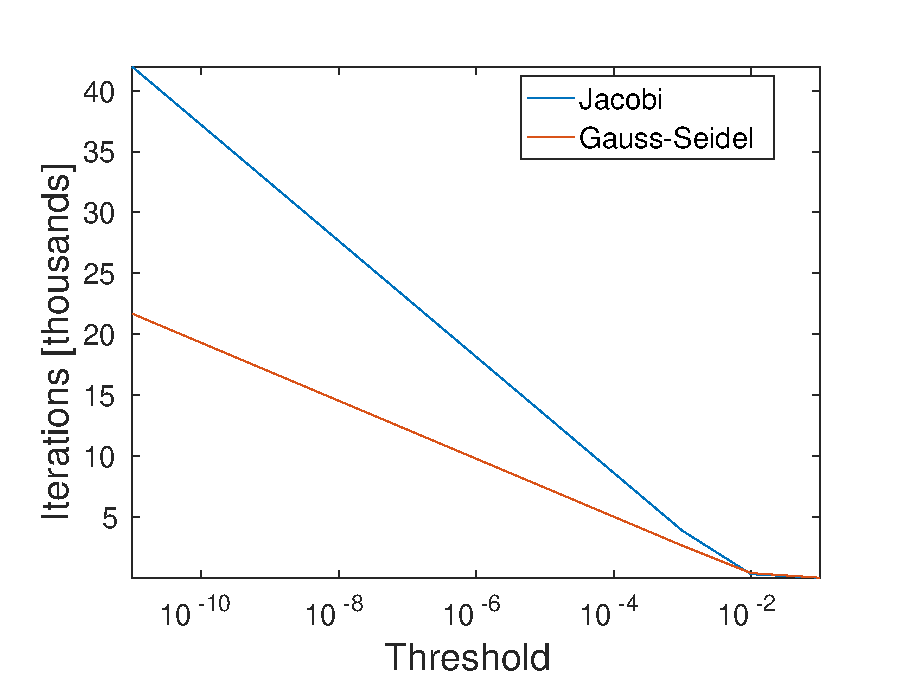
\includegraphics[width = 0.8\textwidth]{fig/itd_jac_gs.eps}
\caption{The convergence of the Jacobi method and the Gauss-Seidel method with changing threshold.}
\label{fig:itd}
\end{figure}

The performance of the two sequential functions are analyzed by comparing the number of point updates per second. The program is forced to run for at least three seconds to get a reliable timing. The resulting graphs is shown in figure \ref{fig:seq_perf}. For small matrices the Jacobi method is $\sim$ twice as fast as the Gauss-Seidel method. This is due to the fact that the Gauss-Seidel method read and write in the same array, which cause some memory "clogging" in the caches. For matrices exceeding the L3 cache, the Jacobi method slows down significantly, due to the smaller bandwidth to/from memory compared to the caches. The Gauss-Seidel method is reduced as well for the same reasons, but not nearly as significantly due to the memory clogging already taking place in the caches. However, as seen on figure \ref{fig:itd}, the Gauss-Seidel method requires half as many iterations to converge to the same precision, making it faster in wall clock time.

\begin{figure}
\centering
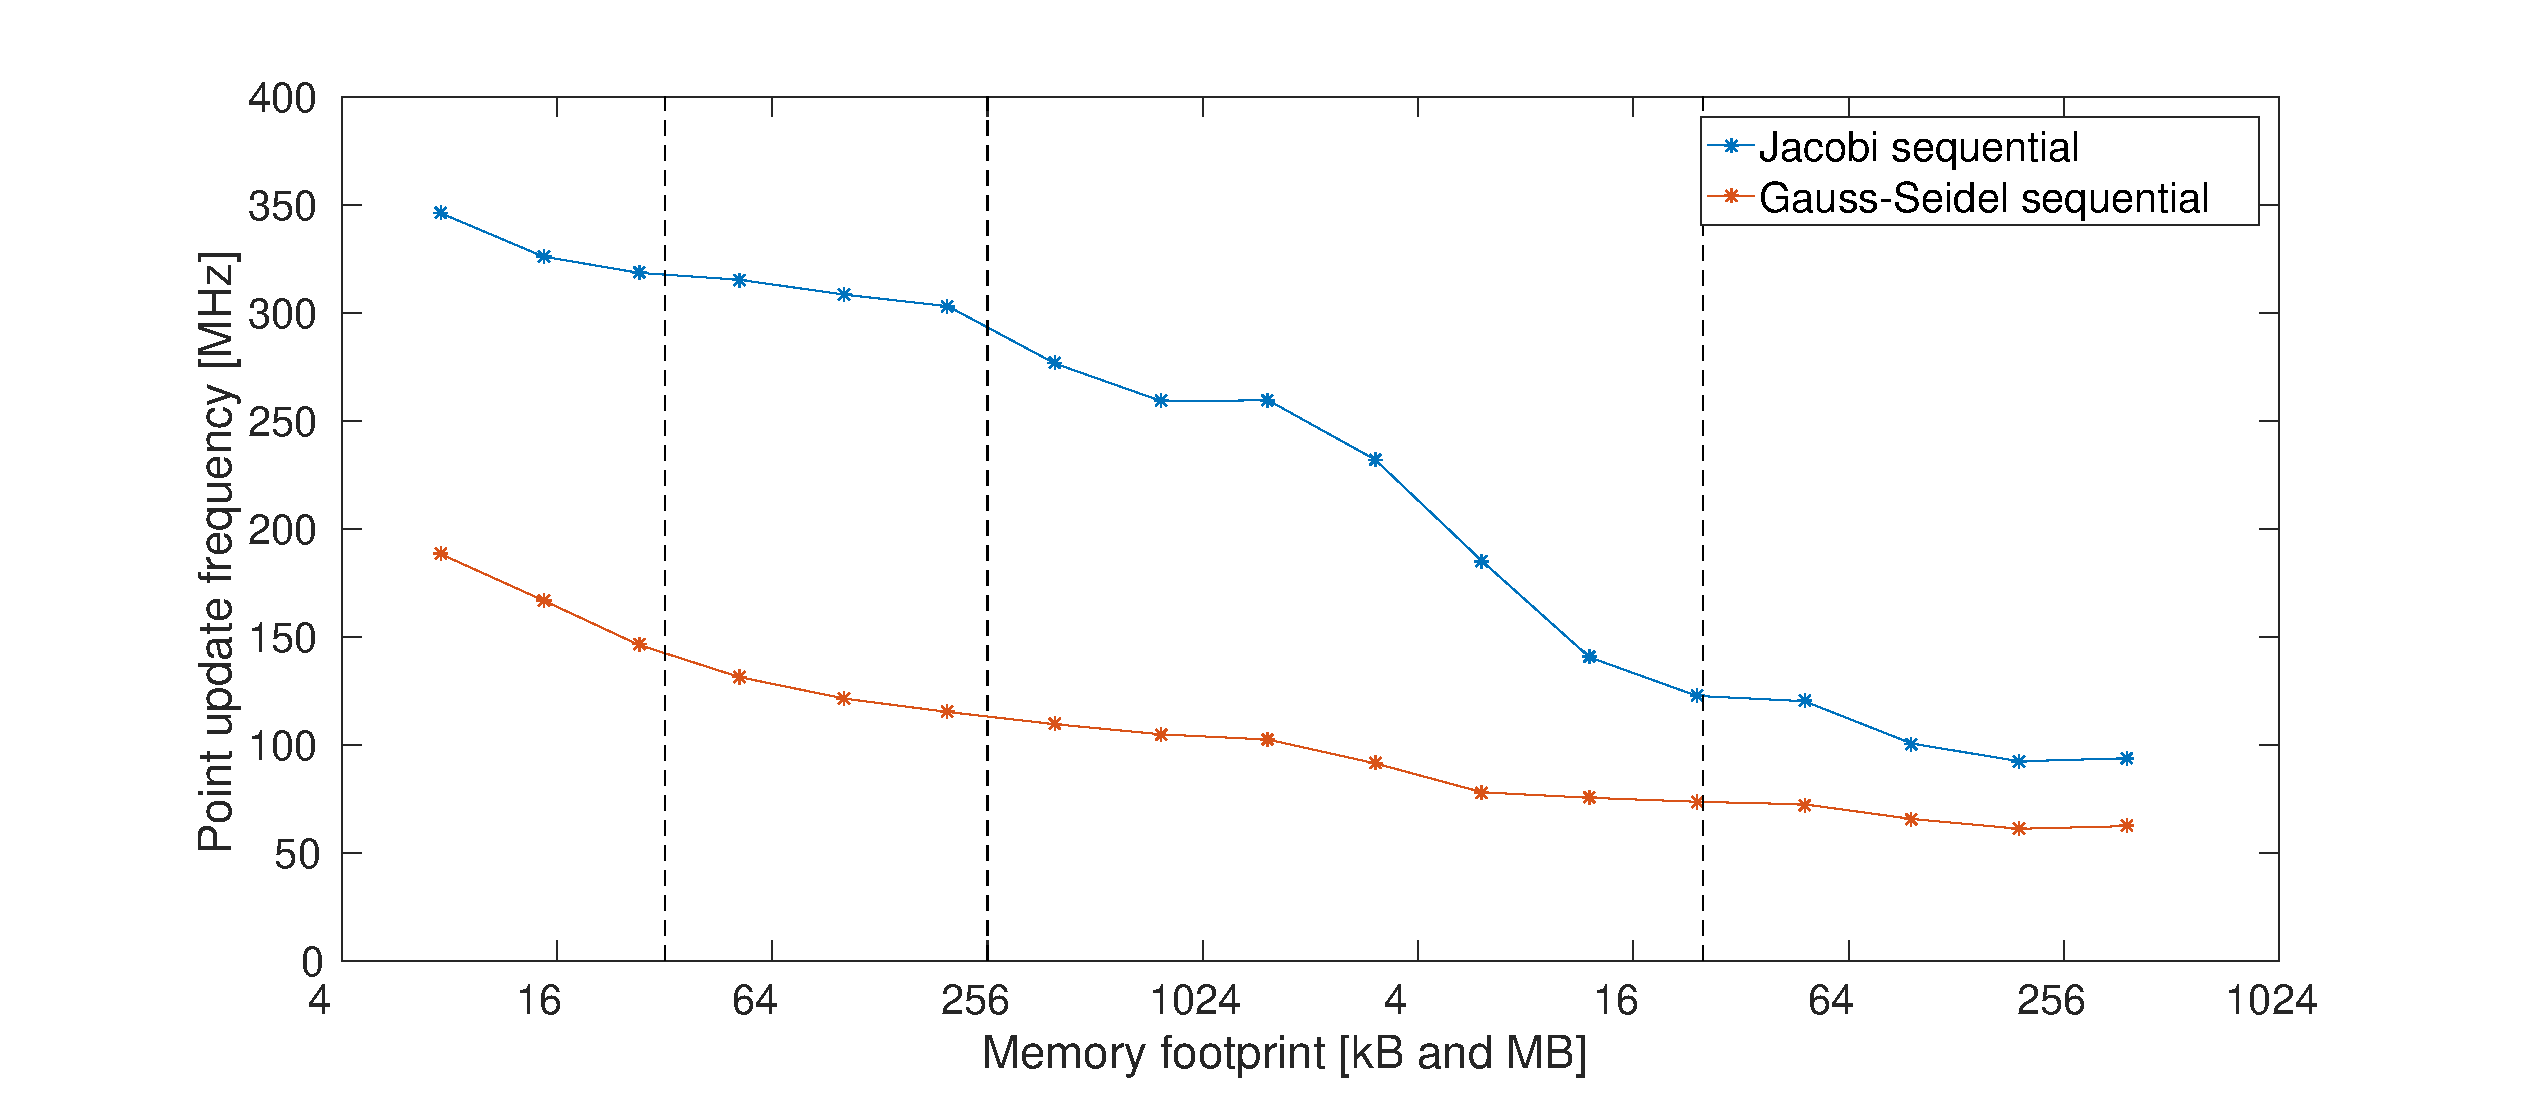
\includegraphics[width = 1.1\textwidth]{fig/seq_perf.eps}
\caption{The performance of the two sequential functions with changing domain size. The black dashed lines represent the cache sizes of the CPU.}
\label{fig:seq_perf}
\end{figure}


\subsection{OpenMP of the Jacobi Method}
The Jacobi method updates a new matrix from the values of an old one, and it is thus easily parallelizable. The program is paralellized using orphaning in openMP. The \texttt{\#pragma omp parallel} is inside the while loop described above. That has the obvious disadvantage that the worker team will be created and destroyed with each iteration, creating a lot of overhead that will reduce performance. To measure and analyze the performance and scaling behavior of the paralized implementations, we map the speedup as a function of the number of processors/threads used. To investigate the speedup, the program is sent through the Sun Studio Performance Analyzer tool in sequential mode to see the fraction of time f spent in the parallelized region, to facilitate a comparison with Amdahl's law. All experiments in this subsection are run with $N = 10000$, $d = 0.01$ and $k_{max} = 10000$. In all cases and with 1 core, the wall time is $\sim 16$ s, verifying that our parallelization does not have any immediate negative effects on our program.

\begin{equation}
S(P)=\dfrac{T(1)}{T(P)}=\dfrac{1}{(f/P+1-f)}
\end{equation}

S(P) is the speed up. T(1) is the sequential execution time, P is the number of processors, T(P) is the execution time on P processors and f is the parallized fraction of the code. The first implementation only parallelizes the Jacobi update loop. So we have a parallel region before the call to jacobi function and a pragma for in the function itself.

\begin{lstlisting}[caption = While loop of our initial omp program]
while(checksum > d && k < kmax){
			#pragma omp parallel default(none) shared(u,uo,f,N,delta2) private(i,j)
			{
				jacobi_seq(u,uo,f,N,delta2);
			} // end parallel
			checksum = fnorm_squared(u,uo,N);
			for(i = 0; i<N; i++){
				for(j = 0; j<N; j++){
					uo[i][j] = u[i][j];
				}
			} 
			
			k++;
		} 
\end{lstlisting}

The speedup of the initial simple implementation is seen in figure \ref{fig:omp_scale1}. It is seen, that we experience some speed up on more processors, but it does stabilize quickly around 5 threads with a speed up factor of 1.15. The f value of 0.22 is found with the analyzer tool, and it is rather low and clearly much of computation time is not spent in parallel, and when we compare it to Amdahl's law, it is clearly not performing well, most likely due to parallel overhead.


\begin{figure}[h!]
\centering
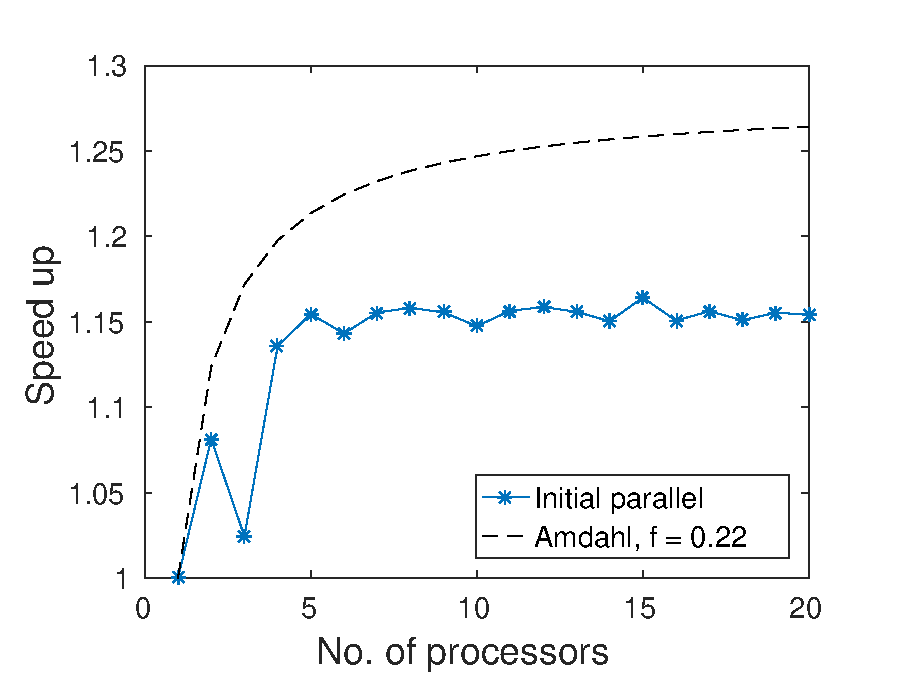
\includegraphics[width = 0.8\textwidth]{fig/speedup_omp.eps}
\caption{Scaling of the first parallelized version.}
\label{fig:omp_scale1}
\end{figure}

We now seek to improve the performance of our OpenMP program. First we realize, that the initial version is only running the Jacobi calculation in parallel, and that the program spent a lot of time on calculating the Frobenius norm and updating the old matrix, about 70 \%. Furthermore, initializing the parallel region in each iteration is not optimal, so we seek to move the parallel region declaration outside the while loop. We created an additional parallel implementation called \texttt{omp2} that deals with these shortcomings. Our while loop for omp2 is as follows.

\begin{lstlisting}[caption = While loop of our optimized (omp2) program]
#pragma omp parallel default(none) shared	(u,uo,f,N,delta2, checksum, k, d, kmax) private(i,j)
				{
				while(checksum > d && k < kmax){
						jacobi_seq(u,uo,f,N,delta2);
						#pragma omp for	private(i,j)  reduction(+:checksum)
						for(i = 1; i <N-1; i++){
							for(j = 1; j<N-1; j++){
								checksum += (u[i][j]-uo[i][j])*(u[i][j]-uo[i][j]);
							}
						}
						#pragma omp for	private(i,j) 
						for(i = 0; i<N; i++){
							for(j = 0; j<N; j++){
								uo[i][j] = u[i][j];
							}
						} 
						#pragma omp master
						{
						k++;
						checksum=checksum/(N*N);		
						}
						#pragma omp barrier
				} // end while 
				
			} // end parallel

\end{lstlisting}


The specific changes are described in the following: The parallel initialization is moved outside the while loop with the shared variables u,uo,f,N,delta2, checksum, k, d and kmax. The Jacobi calculation is parallel using pragma omp for as in the simple version, the checksum is also parallel by using a omp for loop with reduction on checksum, so we do not experience any simultaneous update errors. The update to iteration count k and checksum normalization is inside a pragma omp master directive such that they are only updated once each iteration to ensure the same behavior as the sequential version. In the end we set a barrier to make sure, that the while loop is finished and the loop variables checksum and k updated before starting a new iteration.


We now end up with a much higher parallel fraction f of 0.93, again from the analyzer tool. In figure \ref{fig:omp2_scale} the scaling behavior is seen for the more optimized version. The speed up is clearly much bigger stabilizing at 7 threads with a bit less than a factor 4. It does however not keep up with Amdahl's law, again due to parallel overhead, and the fact that memory initialization is done by the master thread, and used by all threads, which can reduce speedup when the number of cores exceed the number of cores per socket, which in this case is 10.

\begin{figure}[h!]
\centering
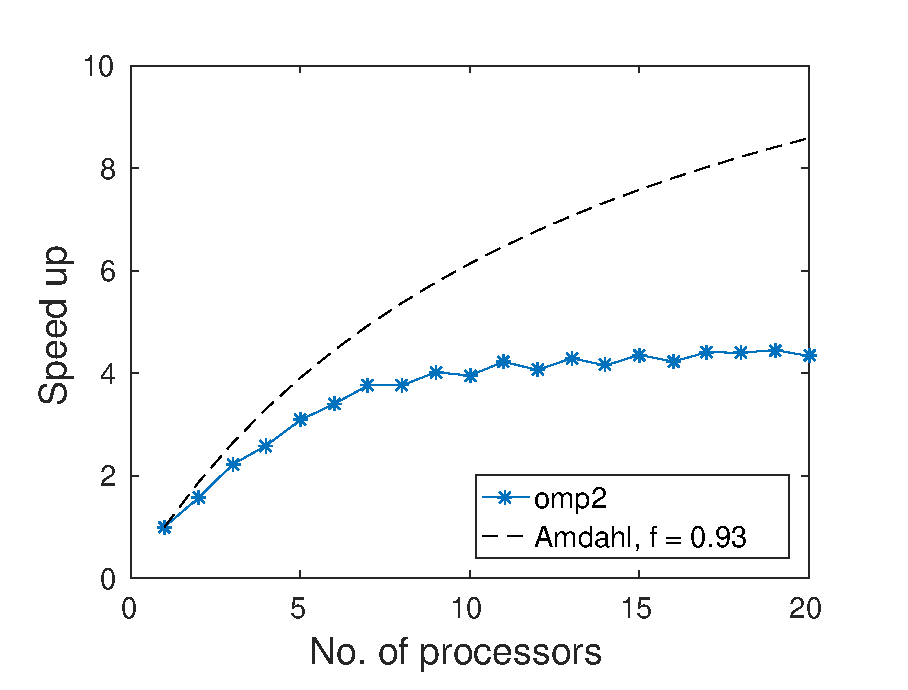
\includegraphics[width = 0.8\textwidth]{fig/speedup_omp2.eps}
\caption{Scaling of the second parallelized version of the whole computational while loop.}
\label{fig:omp2_scale}
\end{figure}

As a final step, we seek to optimize the program even more by implementing a parallelization of the memory allocation and initialization of the matrices to avoid remote memory access when using larger number of threads. This is only relevant when the number of processors exceeds 10 because then processors 10 and above will access data from the other socket. 
We added an if-clause that checks the number of threads and if it is above 10, runs the memory allocation in parallel. We also moved the initialization of the matrices to a parallel region and added pragma fors for the initialization loops.

The way we allocated memory to matrices initially is as follows: 


\begin{lstlisting}[caption = Initial memory allocation]
double ** dmalloc_2d(int m, int n) {
	if (m <= 0 || n <= 0) return NULL;
	double **A = (double **)malloc(m * sizeof(double *));
	if (A == NULL) return NULL;
	A[0] = (double *)malloc(m*n*sizeof(double));
	if (A[0] == NULL) {
		free(A); 
		return NULL; 
	}
	int i;
	for (i = 1; i < m; i++)
		A[i] = A[0] + i * n;
	return A;
}
\end{lstlisting}

With this approach the entire m*n array of matrix values is contiguous meaning everything is stored in a single location.

Since we want different threads to be able to store relevant rows of the matrices to memory locations close to them we need to make sure the calls to malloc are within a parallel region and workshared.
The simplest way to do this is with a pragma omp for as follows:

\begin{lstlisting}[caption = Parallelized memory allocation]

double ** dmalloc_2d_opt(int m, int n) {
	if (m <= 0 || n <= 0) return NULL;
	double **A = (double **)malloc(m * sizeof(double *));
	if (A == NULL) return NULL;
	//A[0] = (double *)malloc(m*n*sizeof(double));	
	#pragma omp parallel default(none) shared (A, m, n)
	{
		int i;
		#pragma omp for	private(i) 
		for (i = 0; i < m; i++)
			A[i] = (double *)malloc(n*sizeof(double));
	}
	return A;
}
\end{lstlisting}


We call this version \texttt{omp3}. The speedup plot can be seen in figure \ref{fig:omp3_scale}. It should be noted that for this plot we fit a line for our speedup curve and computed the f value from the fitted line. Although there is a small dropoff at 19 and 20 threads, the observed f of 0.955 effectively represents the proportion of the problem that we managed to 'perfectly' parallelize.  

As seen from figure \ref{fig:omp3_scale} the increase in speedup continues above 10 processors, which was not the case with \texttt{omp2}.

\begin{figure}[h!]
\centering
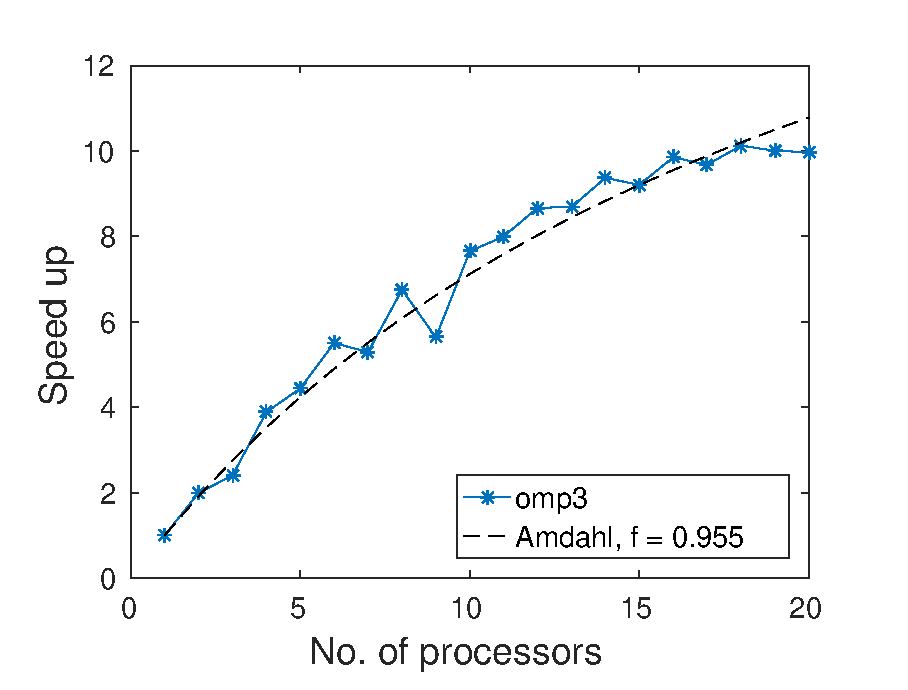
\includegraphics[width = 0.8\textwidth]{fig/speedup_omp3.eps}
\caption{Speed-up scaling of the third parallelized version, which includes parallel memory allocation.}
\label{fig:omp3_scale}
\end{figure}


Lastly, we compare the efficiency of our three different parallel implementations. This is done by computing the efficiency, which is the speed up increase per added thread. Figure \ref{fig:omp_eff} clearly shows how different the efficiency curves are for the three different implementations. The simple implemenation clearly falls of right at the beginning, where the efficiency drops to a little higher than 50\% already at thread nr. 2, which is obvious since the speed up factor is only slightly above 1. For the case of the more optimized implementation, it is clear that the omp3 version reigns supreme, and it does not reach 50\% effiency before the 19th to 20th added thread, which makes sense, since we saw in the speed-up scaling that it started to stagnate at that point. Meanwhile the omp2 parallelization already reaches 50\% around 7-8 threads.

\begin{figure}[h!]
\centering
\includegraphics[width = 0.8\textwidth]{fig/efficiency_omp_omp2_omp3.eps}
\caption{Effiency plot of the three parallel versions.}
\label{fig:omp_eff}
\end{figure}

\subsection{Speedup with varying matrix size}
In this subsection, the speedup of the \texttt{omp3} parallelization is investigated with changing matrix sizes. The threshold level is chosen individually for each size such that the program runs for at least a few seconds. The resulting curves can be seen in figure \ref{fig:speedup_N}. Despite the differing thresholds, the curves are still comparable due to the fact that the parallel region is outside the loop in \texttt{omp3}, which means that each iteration is identical, and so a larger number of iterations does not influence the speedup because it is relative to the case with one processor. The number of iterations for a single curve is constant for all number of processors. For a small number of processors, the speedup is similar, but as the number of processors increase, so does the parallel overhead required to keep track of the threads. This limits the speedup, and for a large number of processors, it even decreases for matrix sizes of $N = 500$ and $N = 1000$. For $N = 100$ the quickest is to use one core, simply because the overhead of even two cores takes more time than is gained by the parallelization. For $N = 10000$ the speedup is not seen to decrease because the matrix is so large that the speed gained from the parallelization is larger than the loss from the parallel overhead. If a larger number of cores was available, a decrease in speedup is expected. For $N = 100$, the analyzer tool was used to confirm our hypothesis: For 1 core, the program took $\sim 2.5$ s to run, but for 10 cores, the program spent 39 s on the implicit barriers after the for loops alone, i.e. a lot of work is done to keep track of the synchronization of the threads while the fraction of time where they are actually working is very small. And that is even when the parallel region is outside the main while loop, so the worker team is not destroyed on each iteration, but it is put to sleep and woken up many times, which also affect performance.
\begin{figure}
\centering
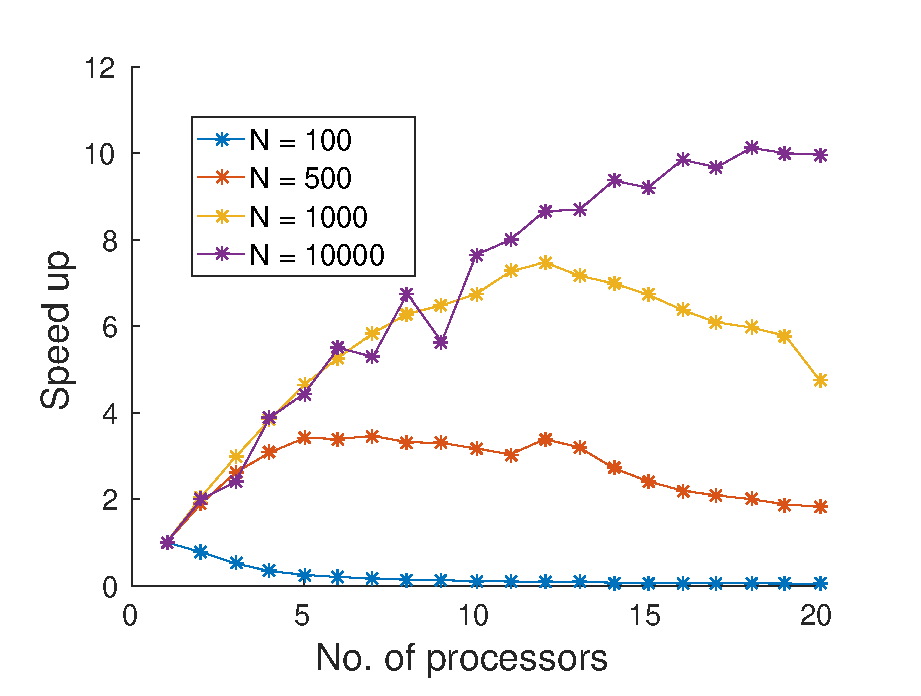
\includegraphics[width = 0.8\textwidth]{fig/speedup_N.eps}
\caption{The speedup of the Jacobi iteration with the best parallellization method, \texttt{omp3}, with different matrix sizes.}
\label{fig:speedup_N}
\end{figure}


\subsection{Speedup with different compiler option}
We now investigate how different compiler options affect the parallelization. The options investigated are \texttt{-fast}, \texttt{-xO3}, \texttt{-xO4}, and \texttt{-xO5}. Optimization levels below 3 is not possible with openMP. The result is seen in figure \ref{fig:compiler}. As can be seen, the wall times vary a bit, but generally speaking, they follow the same trend, irregardless of the compiler optimizations. This is most likely due to the fact that the openMP is processes before the optimizer compiler options. In order to be able to parallelize properly, the openMP outlines loops into functions, such that they can be passed to the worker team, but in turn that also means that the compiler will have a difficult time applying the most advanced optimization schemes as we saw in the exercise calculating pi.

\begin{figure}
\centering
\includegraphics[width = 0.8\textwidth]{fig/compilerOpt.eps}
\caption{The wall times for different number of threads with different compiler optimizations activated.}
\label{fig:compiler}
\end{figure}

\subsection{Comparison with Mandelbrot program}
In this subsection, the scaling of our best parallelized version of the Jacobi method, \texttt{omp3} is compared with the scaling of the computation of the Mandelbrot set. The scaling of the Mandelbrot calculations with a direct implementation and a scheduled version with \texttt{static} with chunk size of 10. The results are shown in figure \ref{fig:mandelbrot} with matrix sizes of 2600 such that in all cases the matrices will only fit in the memory and not the caches. The naive implementation of the Mandelbrot scales badly, especially for a few processors, and better for a larger number of processors. This is due to the fact that when the worker team hits the out for loop in the Mandelbrot program, the columns are divided evenly between the workers, but the work needed to be done is not spread out evenly across the columns. This causes a very imbalanced work distribution, and the resulting speedup is low, only about 50 \% extra for 4 cores compared to 1. For a number of processors larger than 4, the slice of the image each worker gets is so small that more than one worker will work on the heavy section, which causes a speedup of about a factor 2 when going from 4 to 8 cores. However, this comes off a low starting point so it is not too impressive. To mitigate this problem, the worksharing was done with a static schedule with chunk size 10, such that each worker now does columns in chunks of 10, and this causes the work in the computationally heavy region to be spread on all involved processors, giving a near-perfect speedup, as is seen on figure \ref{fig:mandelbrot}. The finally optimized version of the Jacobi method follows the chunked Mandelbrot line when the number of processors are below 5, and then the speedup falls off, to reach a factor of 10 at 20 processors. The difference in speedup can be explained by the fact that the Mandelbrot parallelization is very simple, it only requires a single loop to be parallelized, while the Jacobi method needs quite some work and tricks in order to reach proper scaling. These many loops and opening and closing of parallel regions means that the overhead is much greater in the Jacobi exercise compared to the overhead in the Mandelbrot exercise, which explains why the speedups are similar for a few cores, and not for a large number of cores. The times for the sequential versions of the Mandelbrot and the parallel with 1 cores, was in both cases $\sim 1.4$ s without writing the image to the disc, verifying that the parallization is implemented correctly.

\begin{figure}
\centering
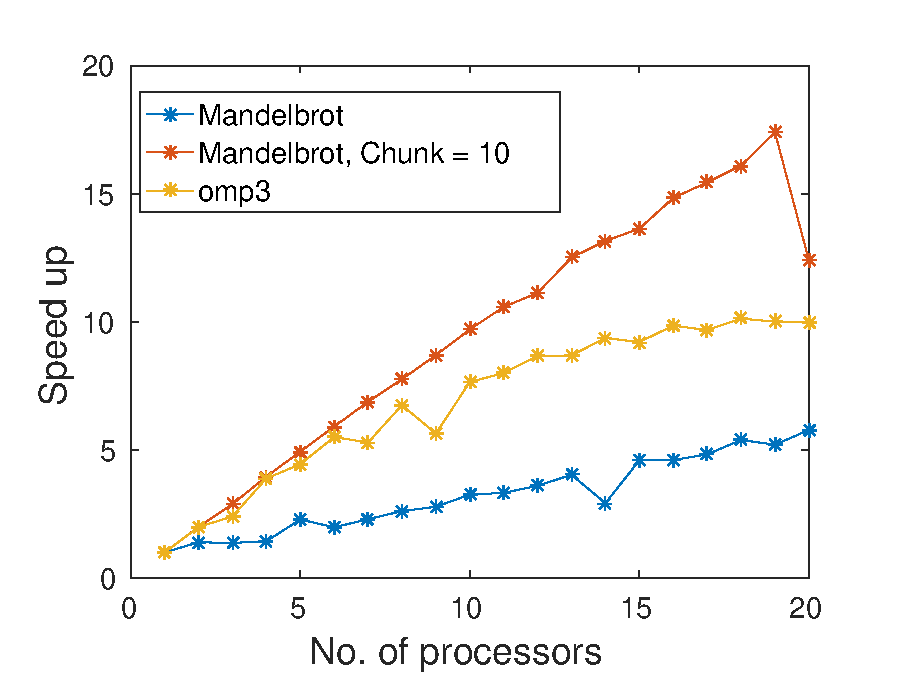
\includegraphics[width = 0.8\textwidth]{fig/mandelbrot.eps}
\caption{The speedup of the two the parallelization of the mandelbrot computation with the default scheduling, with a chunk size of 10 compared to the speedup of the Jacobi iteration.}
\label{fig:mandelbrot}
\end{figure}

\section{OpenMP Gauss-Seidel}
The problem with the Gauss-Seidel smoother is, that it is built around internal data dependencies. It is therefore difficult to implement simple parallelized techniques, since the communication cost between the different threads would be really high. The Jacobi method on the other hand uses another matrix, the u old, which takes up memory space, but it is much easier to feed the data to the threads and finish the computation step. Since implementing a parallelization of the Gauss-Seidel smoothening is more difficult, the Jacobi method or alternatives have been more widely used for multigrid problems.\\

There does however exist modifications to the natural/lexographical version of the Gauss-Seidel smoother, which then seeks parallize using different methods, i.e. blocking. The article by D. Wallin, H. L\"{o}f, E. Hagersten and S. Holmgren\footnote{Dan Wallin, Henrik L\"{o}f, Erik Hagersten and Sverker Holmgren, \textit{Multigrid and GaussSeidel
Smoothers Revisited:
Parallelization on Chip Multiprocessors}, ICS '06 Page 145-155, ACM NY USA, 2006-06-28}  give insight to the complications of the subject and describe both the standard red-black method and their new temporally blocked natural Geiss-Seidel smoother. The completely natural Gauss-Seidel is a single sweep for each step/iteration, and therefore the data is interchanged. The red-black ordering is based on splitting each iteration step up in sweeps, which are fully data parallel. The grid is split into sets of even and odd gridpoints, even points have data dependencies to odd points and vice versa. However, the points do not have dependence to points of the same type. This means a loop over points of the same type can be done in parallel. In practice our initial approach would thus likely be to have a loop over one type of points, then a barrier and then a loop over points of the other type.

Wallin et al succeeded in improving the efficiency up to 40\% compared to some other Gauss-Seidel parallelized smoothers, but it does however depend much on the system and problem at hand.

There exist several possible implementations of the Gauss-Seidel smoother, but it is an evolving field and there exist different approaches. The article by H. Courtecuisse and J. Allard\footnote{Hadrien Courtecuisse, J\'{e}r\'{e}mie Allard, \textit{Parallel Dense Gauss-Seidel Algorithm on Many-Core Processors}, High Performance Computing and Communications, 1th IEEE Conference 2009, IEEE, 2009-06-25} comes with different approaches to the same issue. They present a new parallel dense Gauss-Seidel algorithm, which is based on atomic update counter, which stores an integer counter in shared memory describing the processed blocks. This depends on the system used, but if it is possible on the system, then after an initial delay, the algorithm will get up to speed without facing the huge communication costs. The article further analyzes this algorithm in depth and its performance across different problem parameters and hardware systems.\\





\section{Conclusion}
In this report, a sequential implementation of the Jacobi iterative method and the Gauss-Seidel iterative method was implemented to solve Poisson's differential equation. The Gauss-Seidel method was found to converge twice as few iterations as the Jacobi method, but in turn the grid point updates per second was slower, but in total, the Gauss-Seidel method was found to be quicker in wall clock time. The Jacobi function can be easily parallelized, so three different versions with increasing amount of parallelization was created. The first only parallelized the loop updating each point, which gave a speedup of maximum 15 \%. Secondly, the checking and the iterative while loop was parallelized, which increased the speedup to a factor of $\sim 4$. Finally, the memory allocation and initialization was parallellized, bringing the top speedup to a factor of 10, which corresponds nicely to $f = 0.955$ in Amdahl's law, suggesting that our code has parallelized over 95 \% of the processes. Using this last implementation, it was found that the optimal number of cores used depends on the matrix size due to increasing parallel overhead from an increasing number of cores. Finally, a method for parallelizing the Gauss-Seidel method is discussed, but not implemented.
\end{document}
